\documentclass[a4paper,12pt]{article}

\usepackage[utf8]{inputenc}
\usepackage[english]{babel}
\usepackage{natbib}
\usepackage[T1]{fontenc}
\usepackage{setspace}
\usepackage{graphicx}
\usepackage{hyperref}
\usepackage{csquotes}


\title{Literature Review}
\author{Joshua Bridge \\14032908 \\joshua.m.bridge@stu.mmu.ac.uk}

\pagestyle{headings}

\begin{document}

\maketitle


\tableofcontents

\listoffigures

\doublespacing

\subsection{Introduction}
  In order to understand the background of the technology involved in this project, it is necessary to complete a significant review into the current and past literature. This will help form a basis of knowledge from which the future development and analysis of the proposed system will utilise and build upon. This research will be vital in order to make use of the most optimal technology for any given problem.

  The following review will be an investigation into the current knowledge of the major components of the proposed system, which are as follows:

  \begin{itemize}
    \item The recommendation system.
    \item The image-filter generation system.
    % \item The web-based user interface.
  \end{itemize}

\section{Recommendation systems}
  As defined in \cite{ricci2011introduction}, recommending content is a problem which involves attempting to predict what a user may desire at any given time when using a system. In the ‘internet era’ applications of this are far-reaching, such as recommending products on Amazon.com \cite{linden2003amazon}. Recommendation systems are a popular topic due to the \textquote{abundance of practical applications that help users to deal with information overload and provide personalized recommendations, content, and services to them} \citep{adomavicius2005toward}.

  \cite{jannach2010recommender} describe three different methods for giving recommendations: Collaborative, Collaborative, Content-based, and Hybrid.

  \subsection{Collaborative recommendation}
    When using an online streaming platform that serves video content such as Netflix or YouTube, a user will visit their site looking for something to watch. The problem faced by these sites is trying to find content that the user hasn't seen before, but will align with the user's interests enough to make them want to watch it \citep{davidson2010youtube}, \citep{gomez2016netflix}.
    The information needed to carry out such a prediction can include the semantic value of the entire users history of interaction with the system (often referred to as \textit{metadata} \citep{duval2002metadata}), from which preference can be extrapolated. If there is not enough metadata about the user from which to extrapolate preference with reasonable certainty, then preference can be inferred from other users of the system - especially users with a similar predicted preference.

  \subsection{Content-based recommendation}
    There can sometimes be barriers to using collaborative recommendation, such as when the ‘cold-start problem’ is present. This problem describes when a user has just signed up to a website, it will not yet have enough information / user history to recommend them content \citep{schein2002methods}.
    In this situation content-based recommendation could be used more effectively to build up more reliable recommendations \citep{lops2011content}.
    There are different kinds of content-based recommendation, as it can be applied to many different kinds of content. For example a system may work differently if the content is user-generated as opposed to internally or computer generated, where the information would likely be provided already. In a system with user-generated content, the information about that content would have to be inferred, or provided by the user.

    \subsubsection{Feature extraction for content analysis}
      When content is user-generated and without a definition provided alongside it, its definition must be derived. For textual data this can be done by analysing the words and extrapolating a commonality between keywords to find a prevailing subject \citep{sanderson1999deriving}.
      This type of process is often referred to as ‘Feature extraction’ \citep{guyon2006introduction}.
      When analysing raw data such as an image file or an audio file, this becomes a much more difficult task as you must first find a way of deciphering the content before deriving the subject or meaning.

      Deep learning has recently become a common way of deciphering this content, including for image, audio, and video content types \citep{coates2011analysis}, \citep{ciregan2012multi}, \citep{lee2009unsupervised}, \citep{mobahi2009deep}.
      Spotify has implemented this kind of deep learning to determine genre types from raw audio data - see section \ref{discoverweekly}.
      This can be applied to image data also, for example in the context of a search algorithm, it would bring the most relevant images by content to the top of the results \citep{yee2003faceted}. This works similarly to how a recommender system will select the most relevant items for the user to see.

      Google's ImageNet has proven to be a very reliable system for image classification \citep{krizhevsky2012imagenet}.
      As it has a very high accuracy on most image types, it would be reasonably effective for providing a basis of feature extraction for use in a recommender system. In the system proposed in this report, scene classification along with prevailing colours in the image would be an ideal input into the recommendation system for determining optimal image filters.

      % TODO more on ImageNet

  \subsection{Hybrid recommendation}
    Generally, hybrid recommendation applies both of the previous methods together in order to draw up a more comprehensive list of recommendations, in order to avoid the individual weaknesses of both types.

    \subsubsection{Spotify - Discover Weekly}
    \label{discoverweekly}
      Discover Weekly is a playlist made every week for every user of Spotify. Instead of getting humans to curate a playlist for each and every user, an algorithm is used to try and find a set of songs which it predicts the user will like, but hasn't listened to before. As described by \cite{popper2015dw} it does this by mixing collaborative and content-based recommendation. The first is done by analysing all playlists on spotify and determining their similarity to playlists made by the user. The next step is looking for songs in those playlists that the user in question hasn't heard yet.

      \begin{figure}[ht]
        \centering
        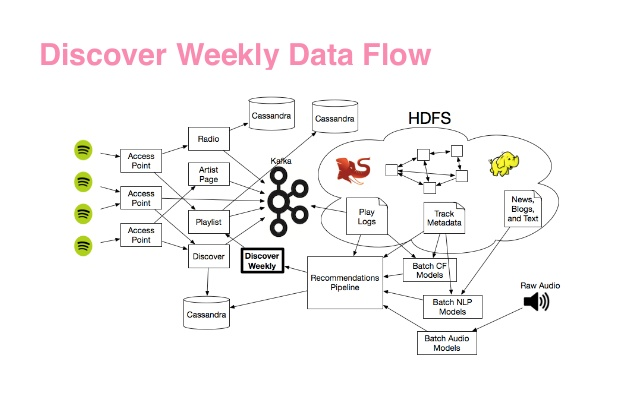
\includegraphics[width=\linewidth]{images/discoverweekly-dataflow}
        \caption[System component architecture of Spotify's ‘Discover Weekly’]{System component architecture of Spotify's ‘Discover Weekly’ \protect\citep{johnson2015dw}}
        \label{fig:discoverweekly-dataflow}
      \end{figure}

      The second, more complicated part of this process is the content-based recommendation. Spotify's algorithms actually analyse the music data in several different ways to determine a users ‘taste’. The first is by defining the genres a user listens to, which it does by scanning music blogs for what genre a certain piece of music is described as being. Using this as a search, spotify can then look for other music in that genre to recommend. The arguably more complicated part of this process is the auditory analysis of raw music data. As shown in figure \ref{fig:discoverweekly-dataflow} the raw audio is converted into ‘batch audio models’ where they can be used as a basis for recommendations.

    % \subsection{Image classification in recommendations}

\section{Image-filter generation}
  There is little to no research into the area of developing new photo filters, likely due to the fact that filters can be very subjective in terms of what effect they have on an image. Furthermore the relation of that effect to how many people choose that filter for a certain type of photograph would require a large data-set. However it is possible to determine the most common types of photographs posted online, which will guide the process of creating filter templates.

  \subsection{Instagram}
    In order to create image filters that users would want to apply to their photographs, an assessment must first be made about that the type of photos people tend to post online. ‘Instagram’ is a popular online photo-sharing platform that attracts over 700 million users \citep{instagram2017users}. An investigation by \cite{hu2014we} revealed that the types of photos posted on Instagram could be roughly categorised into eight types: \textquote{self-portraits, friends, activities, captioned photos (pictures with embedded text), food, gadgets, fashion, and pets}. The study clarifies that ‘self-portraits’ (or ‘selfies’) made up 24.2\% of the images posted, and ‘friends’ made up 22.4\%, totalling 46.6\% of the images analysed. From this it can be hypothesized that creating filters which are complimentary for skin-tones would be a contributing factor to success when developing image-filters.

    \cite{hu2014we} however did not study a wide proportion of the Instagram user-base, in fact they only closely studied 50 users, out of an initial 95,343 ‘unique seed users’, from a user-base of more than 150 million when the study was taken place. Furthermore the study only analyses pictures posted online, to Instagram, with public profiles, and from users which had \textquote{at least 30 friends, 30 followers, and had posted at least 60 photos}. The system proposed in this report would not be limited in terms of where the resulting image would be posted, and has no requirement that the image be posted to an online website. Therefore the findings in the study should only be used as a loose guideline for popular image categories when defining image-filter styles.

  \subsection{Personalisation of image enhancement}
    There has been some work done on the mapping of image enhancement styles to personal taste, although the field appears to be still in early stages. However, two studies in particular have heavily contributed to the development in this field. \cite{kang2010personalization} found that when given a set of images, participants would deviate into different styles when asked to choose between two options of enhancement (e.g. lighter or darker). Furthermore, many participants preferred their own enhancement when compared to an averaged enhancement, suggesting that personalised enhancements would be a valuable tool.

    Using the work done by \cite{kang2010personalization} as a basis, \cite{caicedo2011collaborative} developed a method of personalised image enhancement that focused on putting users into groups (or ‘clusters’) that had similar tastes within image enhancement. Therefore when attempting to apply personalised enhancement on a per-user basis, instead of determining a specific users preference from scratch, the user's preference would only have to be mapped to a pre-defined group. Using this method the authors suggest that personalisation of image enhancement could be scale-able to large amounts of users.

% \section{Web-based user interface}

\newpage
\section{Conclusion}
  Posting images online is fast becoming one of the biggest trends in recent history, as evidenced by Instagram's user-base expanding to over 700 million users \citep{instagram2017users}. While not much public research seems to have been carried out into the reasons why users pick certain styles of image-filters before posting, it certainly appears viable to aid them in making that process easier.
  The findings of this review suggest that feature extraction could be a useful tool in developing recommendations for filters. This would be carried out in the form of image classification, most commonly to determine whether a person is present in a photograph which would thereby influence the algorithm's decision of what filters to recommend to the user for a certain image.

  The findings of this report also suggest (mostly from \cite{kang2010personalization} and \cite{caicedo2011collaborative}) that the field of personalised image enhancements (or filters) is a relatively new field of study, therefore there is a lot of room for collecting new findings by extending upon previous works in a new implementation.

\newpage
\singlespacing

\bibliographystyle{agsm}
\bibliography{literature-review}


\end{document}
